\newcounter{artCounter}
\setcounter{artCounter}{0}
\newcounter{maxArts}
\setcounter{maxArts}{0}

\newcommand{\showLastArt}{\csname artsDef\romannumeral\the\numexpr\arabic{maxArts} - 1\relax\endcsname}

\newcommand{\showArt}{
\csname artsDef\roman{artCounter}\endcsname
\addtocounter{artCounter}{1}
\ifnum \value{artCounter}=\value{maxArts}
\setcounter{artCounter}{0}
\fi
}

\newcommand{\registerArt}[1]{%
\expandafter\newcommand\csname artsDef\roman{maxArts}\endcsname{#1}%
\addtocounter{maxArts}{1}%
}

\registerArt{{
$$ \langle \wedge \ \_\  \wedge \rangle $$
}}

\registerArt{{
$$ \langle Q\ _\perp\ Q \rangle $$
}}

\registerArt{{
$$ \langle Q\ _{^{\dot{\smile}}}\ Q \rangle $$
}}

\registerArt{{
\begin{center}
\begin{tikzcd}[ampersand replacement=\&]
\& *\arrow[ld]\arrow[rd,"h"] \& \& \& *\arrow[ld,swap,"i"]\arrow[rd] \& \\
* \& \& * \& * \& \& * \\
\\
\\
\& \& \phi \arrow[r] \& \theta \& \&
\end{tikzcd}
\end{center}
}}

\registerArt{{
\begin{center}
\begin{tikzcd}[ampersand replacement=\&]
\& *\arrow[ld]\arrow[rd,"h"] \& \& \& *\arrow[ld,swap,"i"]\arrow[rd] \& \\
* \& \& * \& * \& \& * \\
\\
\\
\& \& \phi \arrow[r, bend right=20] \& \theta \& \&
\end{tikzcd}
\end{center}
}}

\registerArt{{
\begin{center}
\begin{tikzcd}[sep=2em,ampersand replacement=\&]
\& *\arrow[ld]\arrow[rd,"h"] \& \& \& \& *\arrow[ld,swap,"i"]\arrow[rd] \& \\
* \& \& * \& \& * \& \& * \\
\\
\\
\& \& \& \phi \arrow[r, loop] \& \& \&
\end{tikzcd}
\end{center}
}}

\registerArt{{
\begin{center}
\begin{tikzcd}[sep=2em,ampersand replacement=\&]
\arrow[dddd, bend right=30]   \pi\& \& *\arrow[ld]\arrow[rd,"h"] \& \& \& \& *\arrow[ld,swap,"i"]\arrow[rd] \& \& \mathcal{H} \arrow[loop right, distance=5em] \arrow[llllllll, dashrightarrow, bend right=25]\\
\& * \& \& * \& \& * \& \& * \&\\
\\
\\
\arrow[rrrrrrrr, dashrightarrow, bend right=20] \theta\& \& \& \& \phi \arrow[r, loop] \& \& \& \& \mathcal{P} \arrow[uuuu, bend right=30]
\end{tikzcd}
\end{center}
}}

\registerArt{{
\begin{center}
\begin{tikzcd}[ampersand replacement=\&]
\& *\arrow[ld]\arrow[rd,"h"] \& \& \& *\arrow[ld,swap,"i"]\arrow[rd] \& \\
* \& \& * \& * \& \& * \\
\\
\& \phi \arrow[rrr,bend right=50] \& \& \& \theta \&
\end{tikzcd}
\end{center}
}}

\registerArt{{
\begin{center}
\begin{tikzcd}[row sep=3em,column sep=3em,ampersand replacement=\&]
\&\&Sa^\prime\arrow[dddd,shorten=21mm,xshift=8mm,yshift=8mm]\arrow[dddd,shorten=21mm,xshift=-8mm,yshift=8mm]\\
\&\&\&\\
Sa\arrow[rrrr,shorten=5em,yshift=1.5mm,leftrightarrow,bend right]\arrow[rruu]\&\&\upsilon\&\&Ta^\prime\arrow[lluu]\\
\&\&\&\&\\
\&\&Ta\arrow[rruu]\arrow[lluu]
\end{tikzcd}
\end{center}
}}

\registerArt{{
\begin{center}
\begin{tikzpicture}
\node at (-1em,0) {(}; 
\node at (1em,0) {)}; 
\node at (0,0) {$\cdot\tau\cdot$}; 
\node[scale=0.5] at (0,-0.5em) {\smile}; 
\end{tikzpicture}
\end{center}
}}

\registerArt{{
\begin{center}
\begin{tikzpicture}
\node at (-1em,0) {(}; 
\node at (1em,0) {)}; 
\node at (0,0) {$\cdot\tau\cdot$}; 
\node[scale=0.5] at (0,-0.5em) {\frown}; 
\end{tikzpicture}
\end{center}
}}

\registerArt{{
\begin{center}
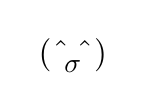
\begin{tikzpicture}
\node[scale=1.2] at (-1em,-0.1em) {(}; 
\node[scale=1.2] at (1em,-0.1em) {)}; 
\node[scale=1.3] at (0,0) {$\hat{}$\ \ $\hat{}$}; 
\node at (0,-0.5em) {$\sigma$}; 
\end{tikzpicture}
\end{center}
}}

\registerArt{{
\begin{center}
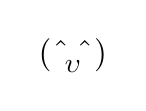
\begin{tikzpicture}
\node[scale=1.2] at (-1em,-0.1em) {(}; 
\node[scale=1.2] at (1em,-0.1em) {)}; 
\node[scale=1.3] at (0,0) {$\hat{}$\ \ $\hat{}$}; 
\node at (0,-0.5em) {$\upsilon$}; 
\end{tikzpicture}
\end{center}
}}

\registerArt{{
\begin{center}
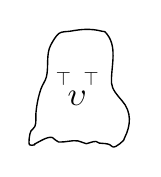
\begin{tikzpicture}
\draw  [xshift=-55,yshift=25,yscale=-0.007,xscale=0.007, color={rgb, 255:red, 0; green, 0; blue, 0 }][line width=0.5] [line join = round][line cap = round] (198,243.5) .. controls (205.86,239.93) and (222.32,228.44) .. (231,231.5) .. controls (235.28,233.01) and (237.48,239.09) .. (242,239.5) .. controls (253.39,240.54) and (266.56,235.76) .. (277,237.5) .. controls (278.29,237.71) and (289.76,241.75) .. (292,242.5) .. controls (293.63,243.04) and (304.42,237.94) .. (310,238.5) .. controls (311.48,238.65) and (314.49,241.28) .. (316,241.5) .. controls (322.04,242.36) and (329.71,241.86) .. (335,244.5) .. controls (338.75,246.37) and (339.71,250.8) .. (346,247.5) .. controls (351.26,244.75) and (355.67,240.56) .. (360,236.5) .. controls (361.31,235.27) and (361.2,233.11) .. (362,231.5) .. controls (373.16,209.17) and (374.98,185.05) .. (357,164.5) .. controls (350.07,156.58) and (338.44,143.93) .. (338,132.5) .. controls (336.8,101.3) and (350.85,64.35) .. (326,39.5) .. controls (324.05,37.55) and (322.52,39.13) .. (320,38.5) .. controls (299.88,33.47) and (283.38,34.98) .. (264,38.5) .. controls (257.75,39.64) and (248.37,38.66) .. (243,42.5) .. controls (236.85,46.89) and (230.44,59) .. (228,63.5) .. controls (218.94,80.22) and (224.47,103.63) .. (220,121.5) .. controls (218.09,129.14) and (212.58,135.75) .. (210,143.5) .. controls (205.3,157.61) and (202.3,171.91) .. (201,187.5) .. controls (200.36,195.13) and (202.08,204.3) .. (199,211.5) .. controls (198.03,213.77) and (192.81,218.36) .. (192,219.5) .. controls (189.31,223.27) and (187.29,242.27) .. (189,244.5) .. controls (191.03,247.14) and (195.67,244.5) .. (199,244.5) ;
\node[scale=0.7] at (0,0) {$\top$\ \ $\top$}; 
\node[scale=1.2] at (0,-0.7em) {$\upsilon$}; 
\end{tikzpicture}
\end{center}
}}

\registerArt{{
\begin{center}
\begin{tikzpicture}
\draw[line width=0.5] [line join = round][line cap = round] \directlua{
math.randomseed(12345)
points = 13
x = 0
y = 0
for i = 0, points - 1 do
  if i == 0 then
    tex.print("(" .. x .. "," .. y .. ")")
  end
  prev_x = x
  prev_y = y
  x = x + 0.1
  y = y + 0.1
  control_x = prev_x + (x - prev_x) / 2
  control_y = prev_y + (y - prev_y) / 2
  r = math.random()
  control_x = control_x + r*0.2
  control_y = control_y - r*0.2
  tex.print(" .. controls (" .. control_x .. "," .. control_y .. ") .. (" .. x .. "," .. y .. ")")
end
};
\end{tikzpicture}
\end{center}
}}